% Elaborado por Fabian Gomez
% Version 1.0

\section{Concept of Operations (ConOps) Summary}\label{sec:conops}

Esta sección resume el Concepto de Operaciones (ConOps) del Rover Olympus y establece cómo se emplea el sistema en el ciclo de vida operativo, con foco en la ejecución del UC‑01 (Exploración de superficie) como caso núcleo de validación en entornos análogos. \cite{segoldmine_ppi, nasa_cm, omg_sysml_mbse}  
El ConOps resume fases de misión, escenarios nominales y contingencias, así como el patrón de interacción Tierra–Rover durante campañas en sitio análogo. El ciclo diario operacional (uplink → ejecución autónoma → downlink → hibernación/idle) se define en §\ref{subsec:daily_ops}. El entorno operacional y las restricciones del sitio análogo se documentan en §\ref{subsec:operational_environment} y §\ref{subsec:operational_constraints}, respectivamente. \cite{segoldmine_ppi, omg_sysml_mbse, nasa_cm}  
El ConOps se utiliza como fuente primaria de derivación y justificación de requisitos (RF/RNF/CON) y como base para la planificación de Verificación y Validación (V\&V) del sistema, manteniendo trazabilidad hacia UC‑01 y los demás Casos de Uso top‑level. \cite{nasa_cm, segoldmine_ppi, omg_sysml_mbse}  

\subsection{Mission Phases (Fases de la Misión)}\label{subsec:mission_phases}
El ciclo de vida operativo se divide en seis fases críticas, desde el aterrizaje hasta el fin de la misión (EOM).

\begin{figure}[H]
    \centering
    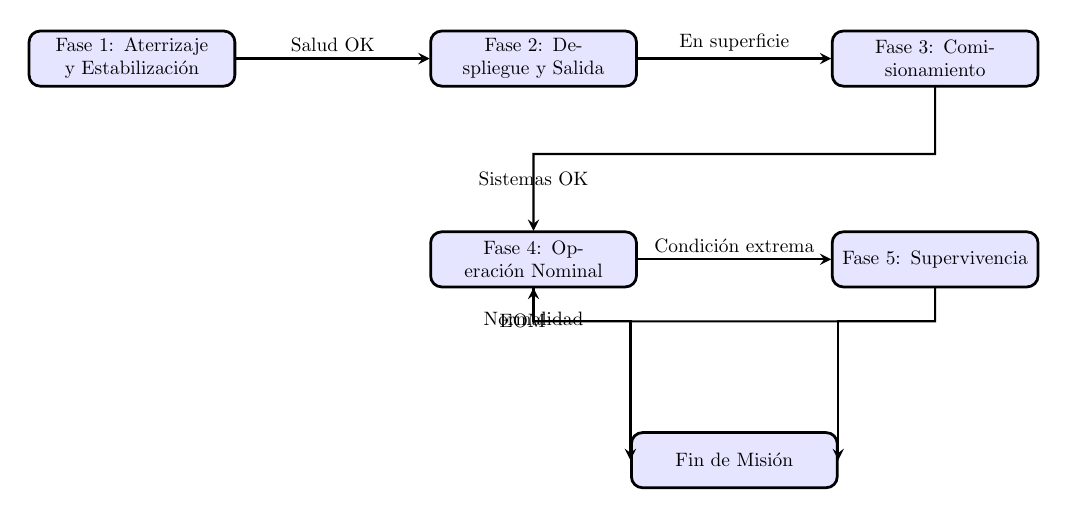
\begin{tikzpicture}[scale=0.85, every node/.style={scale=0.7}]
        \tikzstyle{phase} = [rectangle, draw, fill=blue!10, rounded corners, text width=3.5cm, align=center, minimum height=1cm, line width=1pt]
        \tikzstyle{arrow} = [thick,->,>=stealth]
    
        \node [phase] (landing)    at (0,0)     {Fase 1: Aterrizaje y Estabilización};
        \node [phase] (deploy)     at (6,0)   {Fase 2: Despliegue y Salida};
        \node [phase] (commission) at (12,0)    {Fase 3: Comisionamiento};
        \node [phase] (ops)        at (6,-3)  {Fase 4: Operación Nominal};
        \node [phase] (survival)   at (12,-3)   {Fase 5: Supervivencia};
        \node [phase] (eom)        at (9,-6) {Fin de Misión};
    
        \draw [arrow] (landing) -- (deploy)       node[midway, above] {Salud OK};
        \draw [arrow] (deploy)  -- (commission)   node[midway, above] {En superficie};
        \draw [arrow] (commission.south) -- ++(0,-1) -- ++(-6,0) -- (ops.north) node[pos=0.5, above] {Sistemas OK};
        \draw [arrow] (ops) -- (survival)         node[midway, above] {Condición extrema};
        \draw [arrow] (survival.south) -- ++(0,-0.5) -- ++(-6,0) -- (ops.south) node[pos=0.5, below] {Normalidad};
        \draw [arrow] (ops.south) -- ++(0,-0.5) -| (eom.west) node[pos=0.1, left] {EOM};
        \draw [arrow] (survival.south) -- ++(0,-0.5) -| (eom.east);
    \end{tikzpicture}
    \caption{Ciclo de vida de la misión y transiciones de fase.}
\end{figure}

El ciclo de vida operativo del Rover Olympus se estructura en fases que permiten organizar modos, responsabilidades y criterios de preparación para la validación del UC‑01 en sitio análogo. Las fases se expresan como transiciones lógicas (no como “fases de vuelo” reales), ya que Olympus es una plataforma terrestre de validación. \cite{segoldmine_ppi, nasa_cm, omg_sysml_mbse}  

\begin{itemize}
    \item \textbf{Fase 1: Aterrizaje y Estabilización (análoga / inicialización):} Establecer condición “en superficie” y estabilidad del sistema (energía, cómputo, comunicación). \cite{segoldmine_ppi, omg_sysml_mbse}  
    \item \textbf{Fase 2: Despliegue y Salida:} Habilitar subsistemas críticos (TRAC, PROP, COMMS, GNC, C\&DH) y preparar al rover para iniciar actividades en el entorno análogo. \cite{segoldmine_ppi, nasa_cm}  
    \item \textbf{Fase 3: Comisionamiento:} Calibraciones, chequeos funcionales, verificación de interfaces internas/externas y pruebas previas a operación nominal (pre‑V\&V). \cite{segoldmine_ppi, nasa_cm}  
    \item \textbf{Fase 4: Operación Nominal:} Ejecutar campañas de operación (incluyendo UC‑01 como caso principal), recolectar telemetría y evidencias V\&V, y operar bajo latencia simulada cuando aplique. \cite{segoldmine_ppi, nasa_cm, omg_sysml_mbse}  
    \item \textbf{Fase 5: Supervivencia / Modo Seguro:} Preservar integridad del sistema ante condiciones adversas (p. ej., degradación de enlace, restricciones de energía, condiciones ambientales del sitio) y permitir recuperación a operación nominal cuando sea viable. \cite{segoldmine_ppi, nasa_cm}  
    \item \textbf{Fase 6: Fin de Misión (EOM / Decommissioning):} Cierre controlado de la campaña y transición a un estado final (ver UC‑05 adaptado en §6.2). \cite{segoldmine_ppi, nasa_cm}  
\end{itemize}

\section{System Use Cases}\label{sec:use_cases}

\subsection{Visión general del sistema}\label{subsec:use_cases_overview}
Conforme al contexto del sistema descrito en §\ref{sec:system_context}, los comportamientos esperados del Rover Olympus desde la perspectiva externa se capturan mediante casos de uso de alto nivel para la operación en superficie. Los actores y sistemas externos aplicables (Operador/GCS, Entorno físico e Infraestructura de comunicaciones, entre otros) se definen formalmente en §\ref{subsec:actors_systems}. La lista de casos de uso top-level se presenta en §\ref{subsec:use_cases_top_level}.

\subsection{Casos de uso top-level}\label{subsec:use_cases_top_level}

A partir de la interacción de estos actores con el sistema, se han definido los siguientes casos de uso de alto nivel, los cuales se representan gráficamente en la Figura~\ref{fig:usecase_top}:

\begin{description}
  \item[\textbf{UC-01: Exploración de superficie}] 
 Permite que el rover recorra una región de la superficie de forma autónoma, analizando el terreno, navegando de manera segura y recopilando datos científicos y de navegación. Este caso de uso implica una alta autonomía y es el foco principal del presente trabajo.

  \item[\textbf{UC-02: Navegación dirigida}] 
El rover recibe desde el Operador una orden para desplazarse hasta un punto específico de interés. El sistema calcula y ejecuta la trayectoria hacia ese objetivo, utilizando sus capacidades de navegación y evitación de obstáculos.

  \item[\textbf{UC-03: Recolección de muestras}] 
 El rover recoge muestras del terreno (por ejemplo, suelo o roca), las prepara y las almacena para su análisis posterior, ya sea a bordo o en laboratorios en Tierra. Este caso de uso puede activarse durante la exploración o a partir de una orden directa del Operador.

  \item[\textbf{UC-04: Modo regreso a casa (Homing)}] 
 Permite que el rover regrese a un punto seguro predefinido (por ejemplo, la zona de aterrizaje o una región protegida) cuando se detectan condiciones de riesgo (batería baja, tormentas, pérdida de comunicación prolongada, etc.) o cuando el Operador lo ordena explícitamente.

  \item[\textbf{UC-05: Activar secuencia de autodestrucción (Decommission)}] 
En el caso extremo de fallo crítico o al final de la vida útil de la misión, el rover puede ejecutar una secuencia de autodestrucción o desmantelamiento controlado con el fin de evitar contaminación del entorno o interferencias con futuras misiones.
\end{description}


\begin{figure}[H]
    \centering
    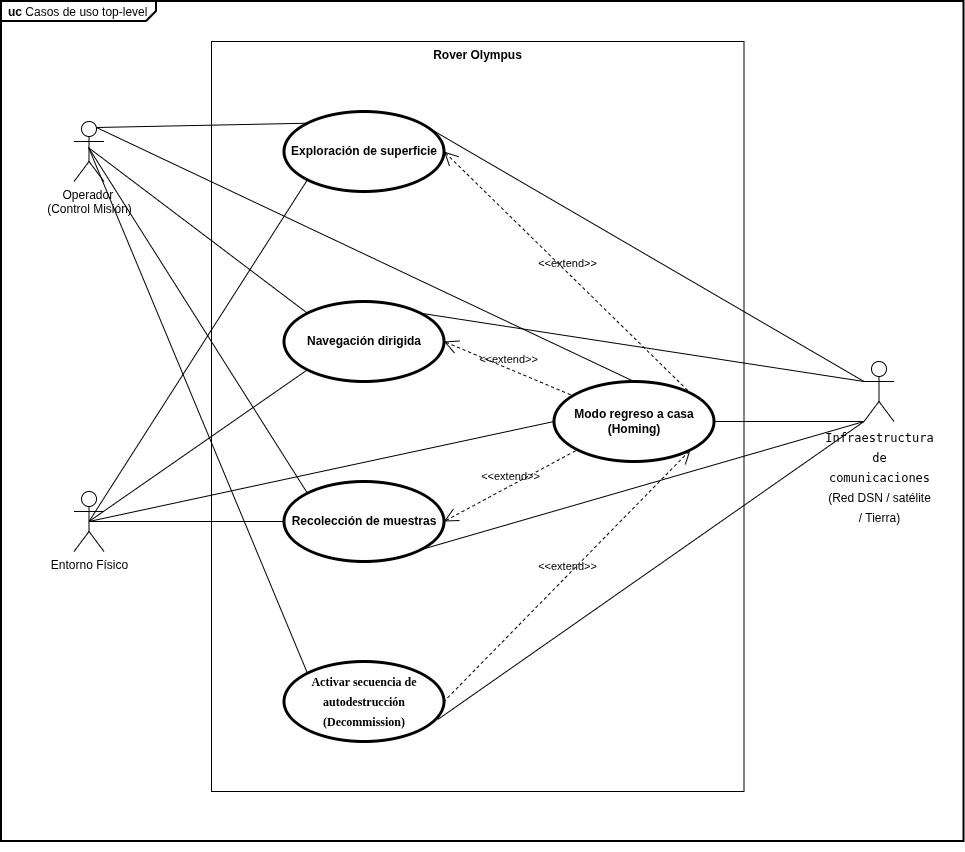
\includegraphics[width=0.5\paperheight]{figures/OLympus USES CASES-USECASE_TOP.drawio.png}
    \caption{Diagrama de Casos de Uso Top-Level: Modos de operación y actores externos.}
    \label{fig:usecase_top}
\end{figure}


Aunque todos estos casos de uso son relevantes para la operación global del Rover Olympus, 
en este documento nos centraremos en el caso de uso \textbf{Exploración de superficie}, 
el cual se detalla a continuación y sirve como base para el modelado de los diagramas de comportamiento.

%---------------------------------------------------------------
\subsection{Caso de uso: Exploración de superficie}\label{sec:uc01}

\subsubsection{Descripción general}\label{subsec:uc01_description}

El caso de uso \textbf{Exploración de superficie} describe cómo el Rover Olympus explora una región del terreno
de forma mayoritariamente autónoma, mientras interactúa con el Entorno físico y con el Operador a través
de la infraestructura de comunicaciones. 

Durante la exploración, el rover:
\begin{itemize}
  \item analiza el terreno y el entorno inmediato,
  \item determina rutas seguras,
  \item navega evitando obstáculos,
  \item recopila y procesa datos científicos y de navegación,
  \item almacena dichos datos para su análisis posterior,
  \item y se comunica periódicamente con el Operador para enviar información y recibir posibles actualizaciones.
\end{itemize}

Este caso de uso es el más complejo de los casos de uso de alto nivel,
ya que integra varios subsistemas (sensado, navegación, gestión de energía, comunicaciones, etc.) 
y exige una toma de decisiones en tiempo real bajo condiciones de entorno cambiantes.

\subsubsection{Actores involucrados}\label{subsec:uc01_actors}
Los actores involucrados en este caso de uso se definen formalmente en §\ref{subsec:actors_systems}. En particular, UC-01 involucra al Operador/GCS como actor primario y al Entorno físico y la Infraestructura de comunicaciones como actores/sistemas externos relevantes (ver §\ref{subsec:actors_systems} y el contexto operacional en §\ref{subsec:operational_context}).

\subsubsection{Objetivo del caso de uso}

El objetivo de \textbf{Exploración de superficie} es permitir que el Rover Olympus explore una región determinada
de la superficie del planeta de forma segura and eficiente, maximizando la cantidad y calidad de datos científicos
recopilados, al mismo tiempo que se preserva la integridad del sistema y se respetan las restricciones de la misión.

\subsubsection{Precondiciones y postcondiciones}

\begin{description}
  \item[\textbf{Precondiciones:}]
  \begin{itemize}
    \item El rover se encuentra en una posición inicial válida dentro de la zona autorizada de exploración.
    \item Los subsistemas críticos (energía, locomoción, sensado y comunicaciones) están operativos.
    \item Existen parámetros de misión definidos por el Operador (zona objetivo, duración máxima, límites de riesgo, etc.).
  \end{itemize}

  \item[\textbf{Postcondiciones de éxito:}]
  \begin{itemize}
    \item La zona de interés ha sido explorada de acuerdo con los criterios establecidos.
    \item Los datos recopilados han sido almacenados a bordo y/o transmitidos a Tierra.
    \item El rover mantiene un estado seguro para continuar con otras operaciones o regresar a un punto seguro.
  \end{itemize}
\end{description}

\subsubsection{Flujo principal de eventos}\label{subsec:uc01_flow}

 El flujo nominal de UC-01 consiste en un ciclo iterativo de (i) recepción de objetivo/parámetros (uplink), (ii) análisis de entorno, (iii) planificación/selección de ruta segura, (iv) navegación con adquisición y gestión de datos, y (v) comunicación periódica de telemetría/datos (downlink), repitiéndose mientras las condiciones sean aceptables. Las decisiones y bifurcaciones (p. ej., ruta no segura, contingencias y salida a modos de seguridad/Homing) se detallan en el diagrama de actividad y su explicación en §\ref{subsec:uc01_activity}.

\subsubsection{Descomposición funcional del caso de uso}

La complejidad de \textbf{Exploración de superficie} se refleja en su descomposición en varios sub-casos de uso
o funciones internas (ver Figura~\ref{fig:usecase_uc01_det}), que se modelan mediante relaciones \texttt{\textless\textless include\textgreater\textgreater} en el diagrama de casos de uso:

\begin{description}
  \item[\textbf{Analizar el terreno}] 
  El rover utiliza sus sensores (cámaras, lidar, etc.) para caracterizar el entorno inmediato, 
  identificando pendientes, rocas, obstáculos y posibles zonas de interés científico.

  \item[\textbf{Recopilar datos del entorno}] 
  Incluye la adquisición de datos científicos (imágenes, espectros, medidas ambientales) 
  y datos de navegación (posición, velocidad, inclinación, etc.).

  \item[\textbf{Procesar la información}] 
  El rover filtra y procesa los datos recopilados para extraer información relevante, 
  como la transitabilidad del terreno, riesgos potenciales o puntos de interés adicionales.

  \item[\textbf{Determinar y navegar por una ruta segura}] 
  A partir de la información procesada, el rover calcula rutas seguras y ejecuta la locomoción a lo largo de dichas rutas,
  ajustando su trayectoria en tiempo real para evitar obstáculos y respetar las restricciones de la misión.

  \item[\textbf{Comunicar con operador}] 
  Comprende el envío periódico de datos y telemetría al Control de Misión, 
  así como la recepción de comandos y actualizaciones de parámetros a través de la infraestructura de comunicaciones.

  \item[\textbf{Evitar obstáculos}] 
  Función especializada que detecta obstáculos en la trayectoria prevista 
  y ejecuta maniobras de evasión manteniendo la seguridad del rover.

    \item[\textbf{Monitorizar estado del rover}] 
  Supervisión continua de variables internas (batería, temperatura, estado de actuadores, integridad de sensores, etc.) 
  para detectar condiciones de riesgo que puedan requerir la activación de un modo seguro o el cambio a otro caso de uso
  (por ejemplo, \textit{Modo regreso a casa}).
  
  \item[\textbf{UC-05: Desactivación segura / Pasivación (Decommission)}] 
  En el caso extremo de fallo crítico o al final de la vida útil de la misión, el rover podrá ejecutar una secuencia de desactivación segura y pasivación, que reduzca a un nivel mínimo los riesgos para el entorno y evite interferencias con futuras misiones, de acuerdo con las consideraciones de protección planetaria aplicables al contexto análogo.
  \end{description}
  

  \begin{figure}[H]
      \centering
      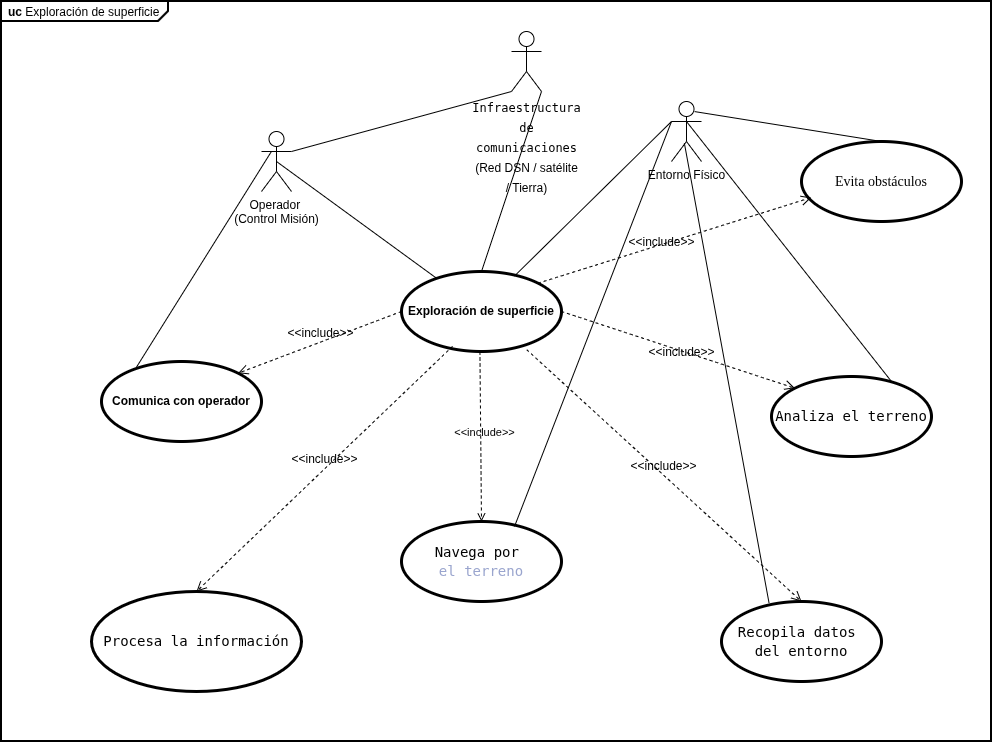
\includegraphics[width=0.5\paperheight]{figures/OLympus USES CASES-Caso_terreno.drawio.png}
      \caption{Descomposición funcional del UC-01: Funciones internas y relaciones de inclusión.}
      \label{fig:usecase_uc01_det}
  \end{figure}

  
  Esta descomposición muestra cómo el caso de uso \textbf{Exploración de superficie} integra múltiples capacidades 
   
del Rover Olympus y justifica que se considere el caso de uso más complejo dentro de las operaciones de superficie.


\subsubsection{Diagrama de actividad del caso de uso ``Exploración de superficie''}\label{subsec:uc01_activity}

El diagrama de actividad asociado al caso de uso \textbf{Exploración de superficie} (ver Figura~\ref{fig:activity_uc01}) modela el
comportamiento dinámico del Rover Olympus cuando se encuentra ejecutando este caso de uso.
Dicho diagrama representa el flujo de acciones que el rover realiza de forma cíclica mientras
explora una región del terreno, así como las decisiones que pueden conducir a la continuación
de la exploración o a la activación de modos de seguridad.

\begin{landscape}
\begin{figure}[H]
    \centering
    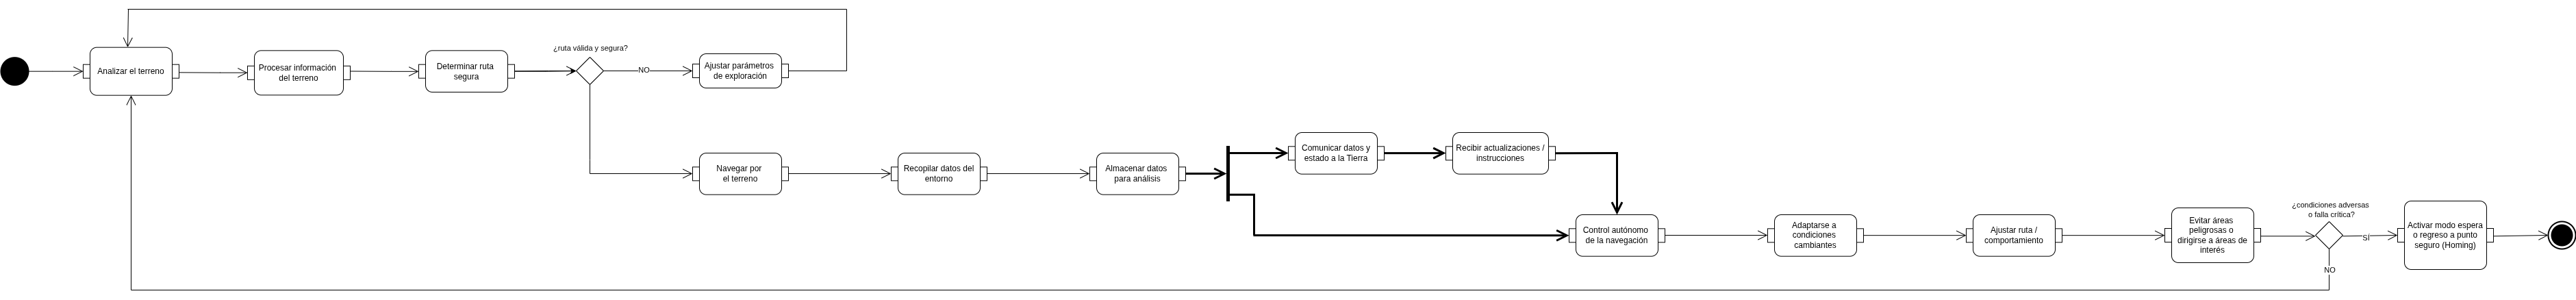
\includegraphics[width=0.8\paperheight]{figures/OLympus USES CASES-activity_diagram.drawio.png}
    \caption{Diagrama de Actividad: Flujo de eventos y toma de decisiones en el UC-01.}
    \label{fig:activity_uc01}
\end{figure}
\end{landscape}

La actividad se inicia cuando el Operador ordena iniciar la exploración de una determinada zona.
A partir de este punto, el flujo principal puede describirse de la siguiente manera:

\begin{enumerate}
  \item \textbf{Analizar terreno}: el rover emplea sus sensores para observar el entorno inmediato y
        caracterizar el terreno (pendientes, obstáculos, zonas transitables, etc.).

  \item \textbf{Procesar información del terreno}: los datos obtenidos se procesan para extraer
        información útil sobre la transitabilidad del terreno y los posibles riesgos.

  \item \textbf{Determinar ruta segura}: con base en la información procesada, el sistema de
        navegación calcula una ruta que cumpla con los criterios de seguridad y las restricciones
        de misión.

  \item \textbf{Decisión: ¿ruta segura?} Si la ruta calculada no se considera segura, el flujo
        pasa a la acción \textit{Ajustar parámetros de exploración}, donde el rover modifica ciertos
        parámetros (por ejemplo, límites de pendiente o distancia a obstáculos) y regresa a
        \textit{Analizar terreno} para replantear la trayectoria. Si la ruta es segura, el flujo
        avanza a la fase de navegación.

  \item \textbf{Navegar por el terreno}: el rover ejecuta los comandos de locomoción para seguir
        la ruta planificada, avanzando por la superficie en dirección a la zona de interés.

  \item \textbf{Recopilar datos del entorno}: durante la navegación, el rover adquiere datos
        científicos (imágenes, medidas ambientales, etc.) y datos de navegación (posición,
        velocidad, inclinación, entre otros).

  \item \textbf{Almacenar datos}: los datos obtenidos se procesan y almacenan en el sistema a bordo
        para su posterior análisis y para su eventual transmisión a Tierra.

  \item \textbf{Ejecución en paralelo (comunicación y control autónomo)}: a continuación, el flujo
        se bifurca mediante un nodo \textit{fork} en dos ramas que pueden ejecutarse en paralelo:
        \begin{itemize}
          \item \textit{Comunicación con la Tierra}: el rover comunica periódicamente datos y
                telemetría de estado al Operador a través de la infraestructura de comunicaciones,
                y puede recibir actualizaciones de parámetros o nuevas instrucciones.
          \item \textit{Control autónomo de la navegación}: el rover controla su navegación de forma
                autónoma, adaptándose a las condiciones cambiantes del entorno, ajustando su ruta
                y su comportamiento, y evitando zonas peligrosas o dirigiéndose a áreas de interés
                científico.
        \end{itemize}
        Una vez completadas ambas ramas, el flujo se sincroniza de nuevo mediante un nodo
        \textit{join}.

  \item \textbf{Decisión: ¿condiciones adversas o falla crítica?} Tras la ejecución paralela, se
        evalúan las condiciones del entorno y el estado interno del rover. Si no se detectan
        condiciones adversas ni fallas críticas, el flujo regresa al paso \textit{Analizar terreno},
        cerrando así el bucle de exploración y permitiendo que el rover continúe explorando de
        forma iterativa.

  \item En caso de que se detecten \textbf{condiciones extremadamente adversas} (por ejemplo,
        tormentas severas, terrenos demasiado peligrosos) o una \textbf{falla crítica} en el
        sistema, el flujo se desvía hacia la acción \textit{Activar modo espera o regreso a punto
        seguro (Homing)}, lo que implica abandonar el ciclo normal de exploración para pasar a un
        modo de seguridad. Este evento marca la finalización de la actividad de exploración de
        superficie y la transición hacia otro comportamiento del sistema centrado en preservar la
        integridad del rover.
\end{enumerate}


\subsubsection{Máquina de estados: Exploración de superficie}\label{subsec:uc01_states}

Esta máquina de estados modela el comportamiento del \textit{Rover Olympus} durante el caso de uso \textit{Exploración de superficie}, describiendo cómo el sistema transita entre \textbf{modos de operación} en respuesta a \textbf{eventos} (triggers) y, cuando aplica, \textbf{guardas} (condiciones booleanas). \cite{UMLStateMachinesConcepts1,UMLStateMachinesConcepts2}

\paragraph{Descripción de la máquina de estados}\label{para:uc01_states_desc}
\begin{sloppypar}
El objetivo del diagrama es representar el ciclo de exploración autónoma
(percepción\allowbreak --\allowbreak planificación\allowbreak --\allowbreak
desplazamiento\allowbreak --\allowbreak adquisición/\allowbreak gestión de
datos\allowbreak --\allowbreak comunicaciones) y los desvíos ante condiciones
adversas (retreat) o fallas críticas (safing).
\cite{UMLStateMachinesConcepts1,UMLStateMachinesConcepts2}
\end{sloppypar}

\textbf{Principio de modelado:}
A diferencia de un diagrama de actividades, una máquina de estados enfatiza los \textbf{estados como condiciones/modos relativamente estables} y las \textbf{transiciones disparadas por eventos}; las acciones internas se expresan como \texttt{entry/} y \texttt{do/} dentro del estado, en lugar de modelarse como estados secuenciales equivalentes a “pasos”. \cite{UMLStateMachinesConcepts1,UMLStateMachinesConcepts2}

\textbf{Nota sobre historia (H):}
El estado compuesto \textit{Exploración activa} incluye un pseudoestado de \textit{historia} (\texttt{H}), utilizado para reanudar el subestado previo del ciclo de exploración tras un \textit{HomingRetreat} cuando las condiciones de riesgo se han normalizado (criterio \textbf{TBD}). \cite{UMLStateMachinesConcepts2}

\begin{landscape}
\begin{figure}[H]
    \centering
    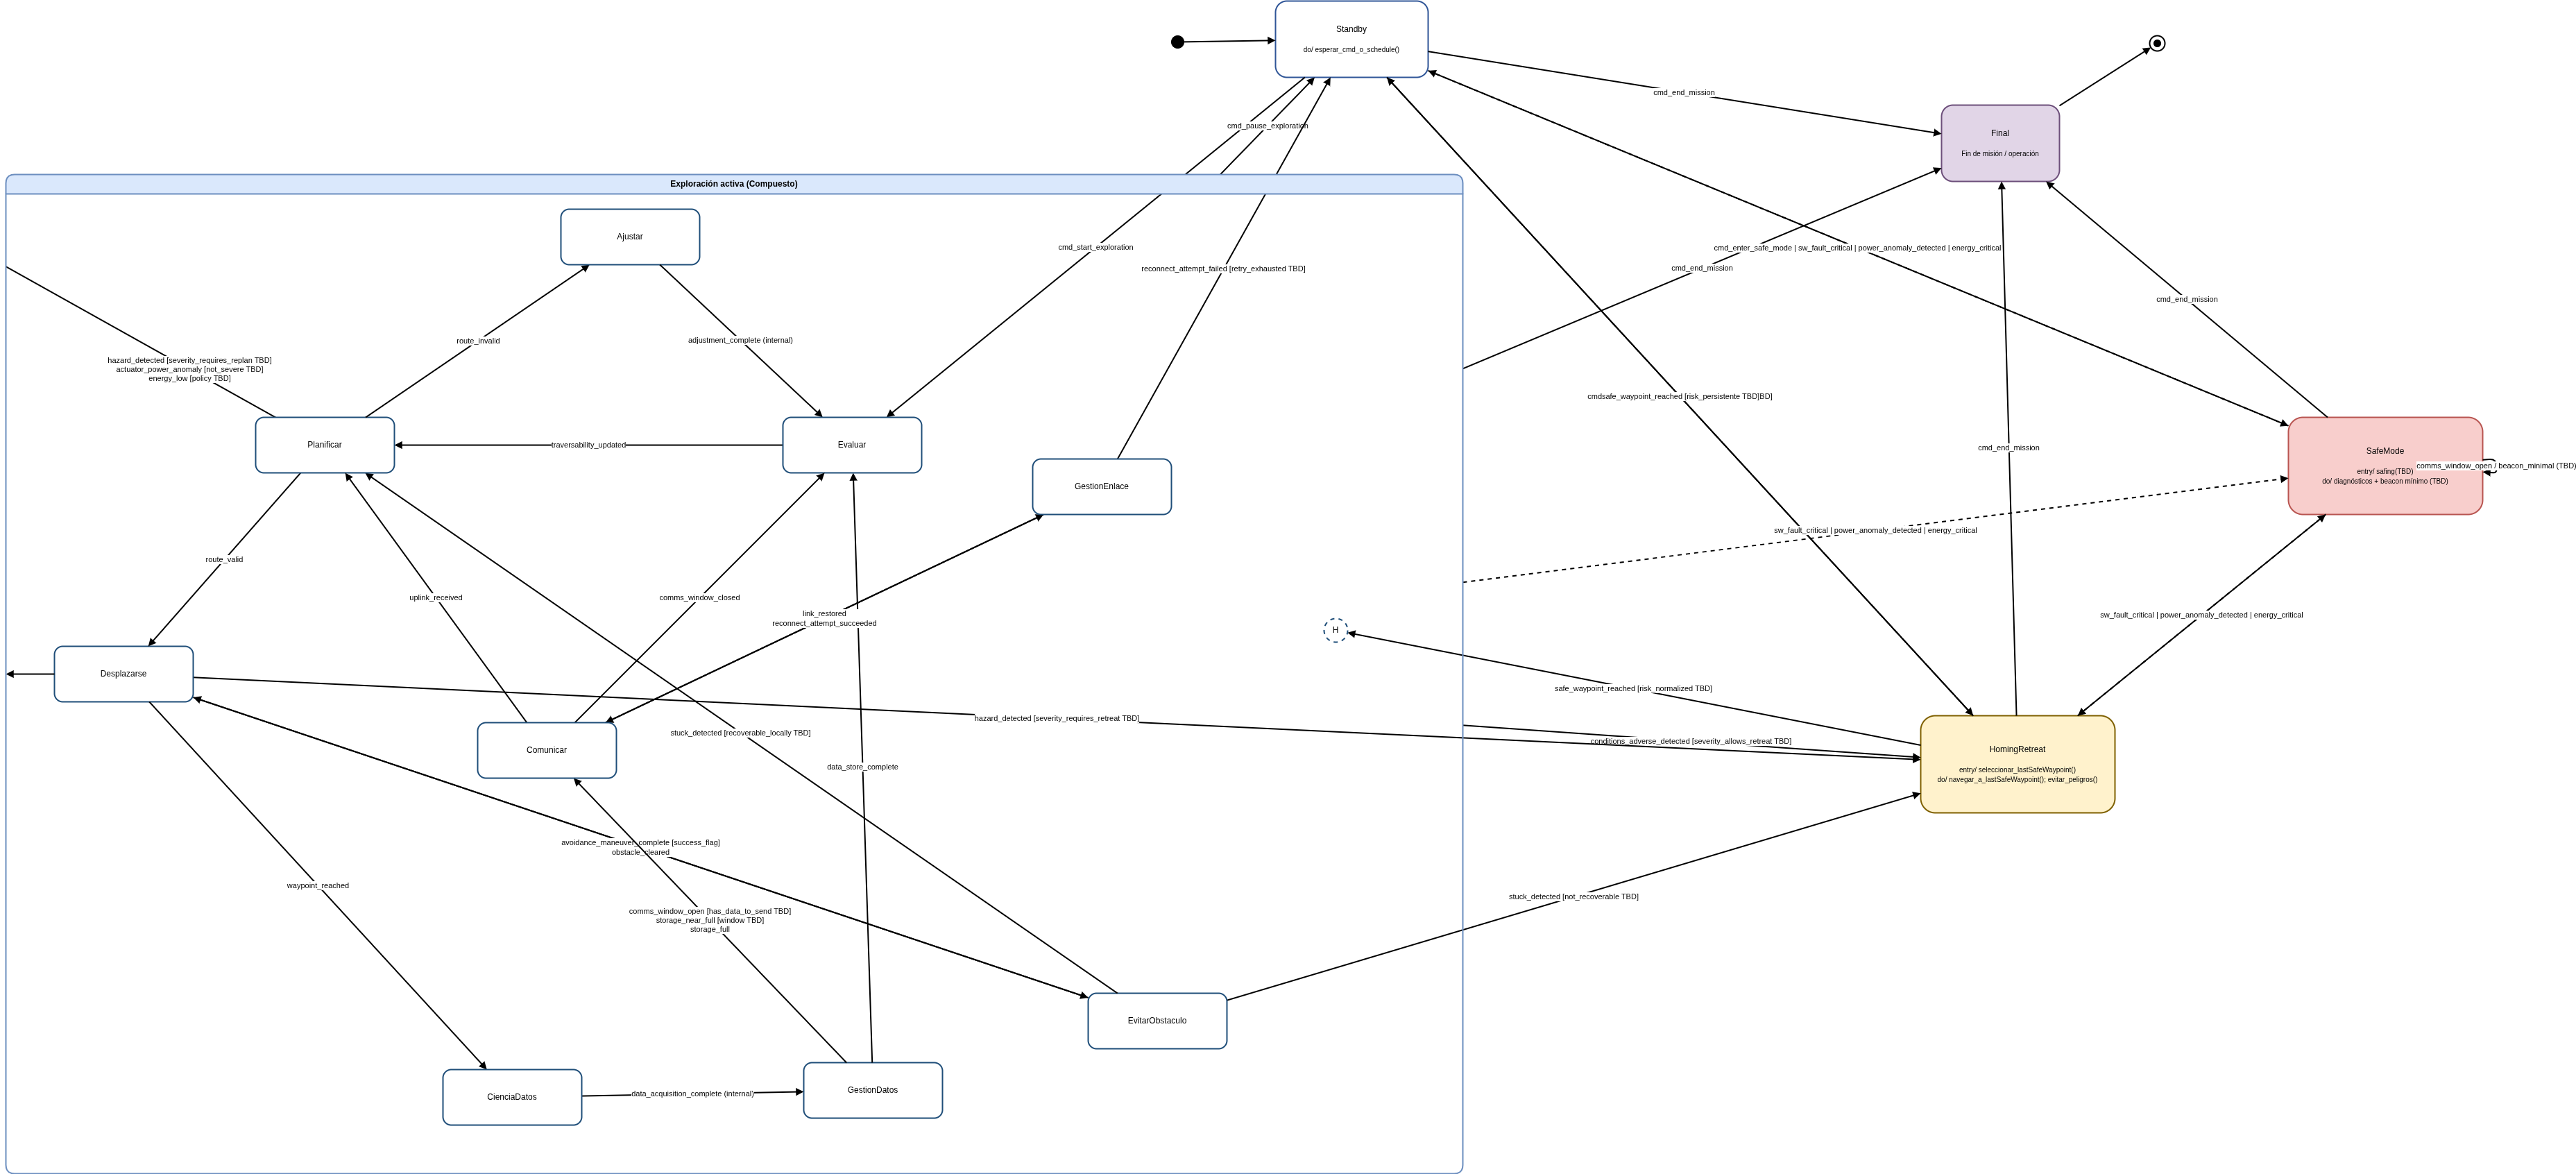
\includegraphics[width=0.85\paperheight]{figures/maquina_lista.drawio.png}
    \caption{Diagrama de la máquina de estados: Modos operacionales y transiciones del Rover Olympus.}
    \label{fig:maquina_estados}
\end{figure}
\end{landscape}

\textbf{Estados top-level (modos de operación):}
\begin{itemize}
  \item \textbf{Standby}: modo de espera operacional; el rover permanece disponible para recibir programación o comandos. Ejecuta \texttt{do/ esperar\_cmd\_o\_schedule()}. \cite{UMLStateMachinesConcepts1}
  \item \textbf{Exploración activa} (estado compuesto): agrupa el ciclo interno de exploración mediante subestados (Evaluar, Planificar, etc.), reduciendo complejidad mediante jerarquía. \cite{CompositeStates1,UMLStateMachinesConcepts2}
  \item \textbf{HomingRetreat}: modo de retirada corta al último waypoint seguro (retreat), usado como respuesta a condiciones adversas. Incluye \texttt{entry/ seleccionar\_lastSafeWaypoint()} y \texttt{do/ navegar\_a\_lastSafeWaypoint(); evitar\_peligros()}. \cite{UMLStateMachinesConcepts2,SafeModeContext1}
  \item \textbf{SafeMode}: modo de preservación (safing), prioriza seguridad del sistema, minimiza actividad no esencial y favorece diagnósticos y comunicación mínima; incluye acciones de \texttt{entry/} y \texttt{do/}. \cite{SafeModeContext1,UMLStateMachinesConcepts2}
  \item \textbf{Final}: término del comportamiento modelado (fin de misión/operación). \cite{UMLStateMachinesConcepts2}
\end{itemize}

\textbf{Eventos y guardas (visión general):}
Las transiciones se disparan por \textbf{eventos} (p.ej.,
\texttt{cmd\_\allowbreak start\_\allowbreak exploration},
\texttt{link\_\allowbreak lost},
\texttt{waypoint\_\allowbreak reached})
y pueden estar condicionadas por \textbf{guardas} (p.ej.,
\texttt{[severity\_\allowbreak allows\_\allowbreak retreat]},
\texttt{[last\_\allowbreak safe\_\allowbreak waypoint\_\allowbreak known]},
\texttt{[has\_\allowbreak data\_\allowbreak to\_\allowbreak send]}).
Las guardas representan condiciones booleanas evaluables; cuando aún no existen
requisitos cuantificados, dichas condiciones se mantienen como \textbf{TBD}
para evitar suposiciones no verificables.
\cite{UMLStateMachinesConcepts2,UMLStateMachinesConcepts1}

\paragraph{Diccionario de eventos (formal)}\label{para:uc01_events}
Este diccionario define un \textbf{subconjunto inicial} de los eventos (triggers) utilizados por la máquina de estados del Rover Olympus para el caso de uso \textit{Exploración de superficie}. 
La información se deriva del BDD (funciones por subsistema). 
Los eventos se especifican como \textit{Command, Signal, Status, Fault, Time}. 
Las condiciones cuantitativas (umbrales, timeouts, políticas) se marcan como \textbf{TBD} hasta disponer de requisitos verificables.
Este diccionario se ampliará para cubrir la totalidad de eventos del diagrama (incluyendo \texttt{cmd\_end\_mission}, \texttt{cmd\_enter\_safe\_mode}, \texttt{energy\_critical}, eventos internos y eventos de recuperación/gestión de enlace). 
Las guardas basadas en severidad (p.\,ej., \texttt{severity\_allows\_retreat}, \texttt{severity\_requires\_replan}, 

\texttt{severity\_requires\_retreat}) y políticas de reintento (\texttt{retry\_allowed}, \texttt{retry\_exhausted}) se consideran TBD y se definirán mediante parámetros configurables en el software, documentados en el ICD de software y reflejados en los procedimientos de prueba correspondientes. Hasta entonces, estas guardas se implementarán como constantes configurables (config files) y su valor por defecto se definirá en la configuración de campaña.

\begin{landscape}
\scriptsize
\renewcommand{\arraystretch}{1.15}
\setlength{\tabcolsep}{3pt}

\begin{longtable}{|p{2.0cm}|p{3.5cm}|p{1.4cm}|p{2.8cm}|p{3.2cm}|p{8.5cm}|}
\caption{Diccionario de eventos (formal) — Rover Olympus}\label{tab:diccionario_eventos}\\
\hline
\textbf{ID} & \textbf{Evento} & \textbf{Tipo} & \textbf{Origen} & \textbf{Consumidor(es)} & \textbf{Descripción / Efecto esperado / Datos (payload)} \\
\hline
\endfirsthead

\hline
\textbf{ID} & \textbf{Evento} & \textbf{Tipo} & \textbf{Origen} & \textbf{Consumidor(es)} & \textbf{Descripción / Efecto esperado / Datos (payload)} \\
\hline
\endhead

\hline
\multicolumn{6}{r}{\textit{Continúa en la siguiente página}}\\
\endfoot

\hline
\endlastfoot

% ---- Modo/Operación ----
EVT-CMD-001 & cmd\_start\_exploration & Command & Operator/\allowbreak COMMS/\allowbreak C\&DH & C\&DH, GNC, COMMS, EPS & 
Inicia Exploración de superficie. Efecto: Standby $\rightarrow$ ExploracionActiva. 
Payload: mission\_phase, area\_of\_interest\_id, policy\_id(\textbf{TBD}), constraints\_ref(\textbf{TBD}). \\
\hline

EVT-CMD-002 & cmd\_pause\_exploration & Command & Operator/\allowbreak COMMS/\allowbreak C\&DH & C\&DH, GNC &
Pausa exploración (no SafeMode). Efecto: ExploracionActiva $\rightarrow$ Standby (o Paused opcional). 
Payload: reason\_code, resume\_policy(\textbf{TBD}). \\
\hline

EVT-CMD-004 & cmd\_homing\_retreat & Command & Operator o lógica (C\&DH/GNC) & GNC, TRAC, PROP &
Retreat al último waypoint seguro (Homing A). Efecto: ExploracionActiva $\rightarrow$ HomingRetreat.
Payload: last\_safe\_waypoint\_id, retreat\_policy\_id(\textbf{TBD}). \\
\hline

EVT-STS-003 & conditions\_adverse\_detected & Signal & GNC/EPS/C\&DH & StateMachine &
Condiciones adversas detectadas (definición \textbf{TBD}). Efecto: ExploracionActiva $\rightarrow$ HomingRetreat.
Payload: cause\_hint(\textbf{TBD}), severity(\textbf{TBD}). \\
\hline

% ---- COMMS ----
EVT-COM-001 & comms\_window\_open & Status & COMMS & C\&DH, StateMachine &
Ventana de comunicación disponible. Efecto: habilita/activa estado Comunicar si hay datos/telemetría.
Payload: window\_id, duration(\textbf{TBD}). \\
\hline

EVT-COM-004 & link\_lost & Fault & COMMS & C\&DH, StateMachine &
Pérdida de enlace detectada. Efecto: transición a \texttt{GestionEnlace} y degradación según política (\textbf{TBD}).
Payload: last\_link\_quality(\textbf{TBD}), timestamp, cause\_hint(\textbf{TBD}). \\
\hline

EVT-COM-005 & link\_restored & Status & COMMS & C\&DH, StateMachine &
Enlace recuperado. Efecto: salir de Recovery $\rightarrow$ Comunicar o retomar ciclo.
Payload: link\_quality(\textbf{TBD}), timestamp. \\
\hline

EVT-COM-009 & uplink\_received & Signal & COMMS & C\&DH, StateMachine &
Uplink recibido (comandos/actualizaciones). Efecto: C\&DH enruta cmd\_received/cmd\_routed; puede disparar replanificación.
Payload: cmd\_batch\_id, priority(\textbf{TBD}). \\
\hline

% ---- C&DH ----
EVT-CDH-003 & telemetry\_due & Time & C\&DH & StateMachine, COMMS &
Telemetría/logs deben emitirse. Efecto: preparar downlink\_ready; priorizar Comunicar si hay ventana.
Payload: tm\_profile\_id(\textbf{TBD}), log\_level(\textbf{TBD}). \\
\hline

EVT-CDH-007 & storage\_near\_full & Status & C\&DH & StateMachine, COMMS &
Almacenamiento cercano al límite. Efecto: priorizar downlink / compresión / retención según política (\textbf{TBD}).
Payload: free\_space\_bytes, percent\_free. \\
\hline

EVT-CDH-010 & sw\_fault\_critical & Fault & C\&DH & StateMachine, EPS, COMMS &
Falla lógica crítica. Efecto: Any $\rightarrow$ SafeMode. Payload: fault\_code, module\_id, severity, evidence\_ref(\textbf{TBD}). \\
\hline

% ---- GNC ----
EVT-GNC-008 & route\_valid & Status & GNC & StateMachine, TRAC, PROP &
Ruta válida/segura (criterio \textbf{TBD}). Efecto: Planificar $\rightarrow$ Desplazarse.
Payload: route\_id, risk\_score(\textbf{TBD}). \\
\hline

EVT-GNC-010 & waypoint\_reached & Status & GNC & StateMachine, C\&DH &
Waypoint alcanzado. Efecto: Desplazarse $\rightarrow$ Ciencia/Datos o Gestión de datos.
Payload: waypoint\_id, pose\_estimate, timestamp. \\
\hline

% ---- Obstáculos ----
EVT-MOB-001 & obstacle\_detected & Signal & GNC & StateMachine &
Obstáculo detectado. Efecto: Desplazarse $\rightarrow$ EvitarObstaculo.
Payload: obstacle\_id(\textbf{TBD}), relative\_pose(\textbf{TBD}), severity(\textbf{TBD}). \\
\hline

% ---- EPS/PROP ----
EVT-EPS-005 & power\_anomaly\_detected & Fault & EPS & StateMachine, C\&DH, PROP &
Condición eléctrica anómala. Efecto: aislamiento de segmento o SafeMode según política (\textbf{TBD}).
Payload: anomaly\_type(\textbf{TBD}), bus\_id(\textbf{TBD}), measured\_values(\textbf{TBD}), timestamp. \\
\hline

\end{longtable}
\end{landscape}



\subsubsection{Daily Operations Cycle (Ciclo Diario)}\label{subsec:daily_ops}

El ciclo diario operacional describe el patrón típico de interacción entre GCS (operador) y el Rover Olympus durante campañas en sitio análogo. \cite{segoldmine_ppi, omg_sysml_mbse, nasa_cm}  

\begin{enumerate}
    \item \textbf{Uplink (Planificación / Comandos):} El operador envía objetivos o comandos de alto nivel (p. ej., meta/área a explorar) y parámetros de ejecución. \cite{segoldmine_ppi, nasa_cm}  
    \item \textbf{Ejecución autónoma (ELANav):} El rover ejecuta navigation autónoma local (percepción, clasificación de transitabilidad, evitación, compensación de slip) y gestiona contingencias (fault stop, retorno a comunicación). \cite{segoldmine_ppi, nasa_cm, omg_sysml_mbse}  
    \item \textbf{Downlink (Telemetría / Datos):} El rover transmite telemetría y datos de desempeño (logs, estados, métricas relevantes) para análisis posterior. \cite{nasa_cm, segoldmine_ppi, omg_sysml_mbse}  
    \item \textbf{Hibernación / Idle:} El rover entra en un modo de bajo consumo o reposo operativo entre ventanas de actividad o condiciones del sitio. \cite{segoldmine_ppi, nasa_cm}  
\end{enumerate}

\begin{figure}[H]
    \centering
    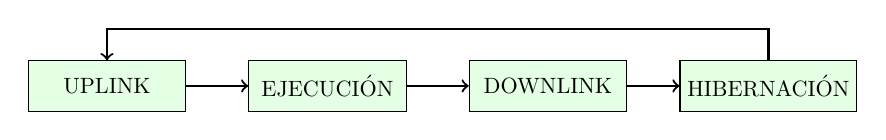
\begin{tikzpicture}[scale=0.8, every node/.style={scale=0.8}]
        \tikzstyle{act} = [rectangle, draw, fill=green!10, minimum width=2.5cm, minimum height=0.8cm]
        \node [act] (up) at (0,0) {UPLINK};
        \node [act] (ex) at (3.5,0) {EJECUCIÓN};
        \node [act] (dw) at (7,0) {DOWNLINK};
        \node [act] (sl) at (10.5,0) {HIBERNACIÓN};
        \draw [thick,->] (up) -- (ex); \draw [thick,->] (ex) -- (dw); \draw [thick,->] (dw) -- (sl);
        \draw [thick,->] (sl.north) -- ++(0,0.5) -| (up.north);
    \end{tikzpicture}
    \caption{Ciclo diario típico: Interacción Tierra-Rover.}
\end{figure}

\subsubsection{Operational Context Diagram (Contexto Operacional)}\label{subsec:operational_context}

 El contexto operacional para UC-01 consolida las entidades externas y las interfaces principales durante operación en sitio análogo. La frontera del sistema y entidades externas se definen en §\ref{subsec:system_boundary}, y los actores/sistemas externos se detallan en §\ref{subsec:actors_systems}. Este diagrama resume dichas relaciones para facilitar la lectura del UC-01 y su interacción TM/CMD. [6, 3, 7]

\begin{figure}[H]
    \centering
    \begin{tikzpicture}[node distance=3cm, auto, scale=0.7, every node/.style={scale=0.7}]
      \node [rectangle, draw, fill=orange!5, text width=3cm, align=center, minimum height=1.2cm] (op) at (5,0) {Operador\\(Estación Control)};
      \node [ellipse, draw, fill=gray!5, text width=2.5cm, align=center] (env) at (0,3) {Entorno\\(Terreno)};
      \node [rectangle, draw, fill=blue!5, text width=3.5cm, align=center, minimum height=1.5cm, line width=1.5pt] (rov) at (0,0) {\textbf{ROVER OLYMPUS}};
      \node [rectangle, draw, fill=green!5, text width=2.5cm, align=center] (com) at (-5,0) {Infraestructura\\Enlace};
      \draw[<->, thick] ( rov.east) -- (op.west) node[midway, above] {TM/CMD};
      \draw[->, thick] (env) -- (rov.north) node[midway, right] {Física};
      \draw[<->, thick] (rov.west) -- (com.east) node[midway, above] {Link};
    \end{tikzpicture}
    \caption{Diagrama de contexto: Entidades externas e interfaces de misión.}
\end{figure}

\subsubsection{Operational Constraints in Analog Sites}\label{subsec:operational_constraints}

Las siguientes restricciones operacionales describen condiciones específicas del sitio análogo que deben considerarse durante operación y validación:


\begin{enumerate}
    \item \textbf{Geometría y mecánica del terreno:} Pendientes de hasta 20° y transiciones de suelo con obstáculos;estas condiciones pueden inducir slip y atascos (ver caracterización del entorno en §\ref{subsec:operational_environment}).\cite{segoldmine_ppi, nasa_cm, omg_sysml_mbse}  
    \item \textbf{Iluminación y visibilidad:} Presencia de zonas de sombra o baja iluminación que afecta percepción visual y clasificación de transitabilidad (ver §\ref{subsec:operational_environment}). \cite{omg_sysml_mbse, segoldmine_ppi}  
    \item \textbf{Comunicaciones con latencia simulada (CON‑002):} Inyección de latencia 0–5 s en el enlace para emular retardo operacional (ver §\ref{subsec:operational_environment} y CON-002 en requisitos). \cite{nasa_cm, segoldmine_ppi}  
    \item \textbf{Condiciones de campaña “lab‑only” (CON‑001):} Marco operativo controlado donde la restricción energética se simplifica respecto a una misión espacial real (ver CON-001 en requisitos).. \cite{nasa_cm, segoldmine_ppi}  
\end{enumerate}
